\documentclass[12pt]{article}
\usepackage[left=0.5in, right=0.5in, top=0.75in, bottom=0.5in]{geometry}
\usepackage{epsfig,graphics,amsmath,color,multicol,enumitem,tabularx,pbox,url}
\usepackage{cancel}
%\usepackage[firstpage]{draft watermark}

\setlist{noitemsep}
\setlist{nolistsep}

\pagestyle{empty}

\begin{document}


\begin{tabular*}{\textwidth}{@{\extracolsep{\fill}}l l}
\textbf{Second Derivative}  &  Wizard name: \hrulefill \\
%\textbf{\today} & MATH 157, Hogwart's House: \rule{4cm}{0.5pt}  \\
\textbf{Math 160 } & MATH 160 Hogwart's House:\hspace{2cm} \\
\hline\hline
\end{tabular*} 

\normalsize 

\section*{Motivating Second Derivatives of Functions}
Using the graph of $f(x)$ below, work through the following questions
\begin{center}
    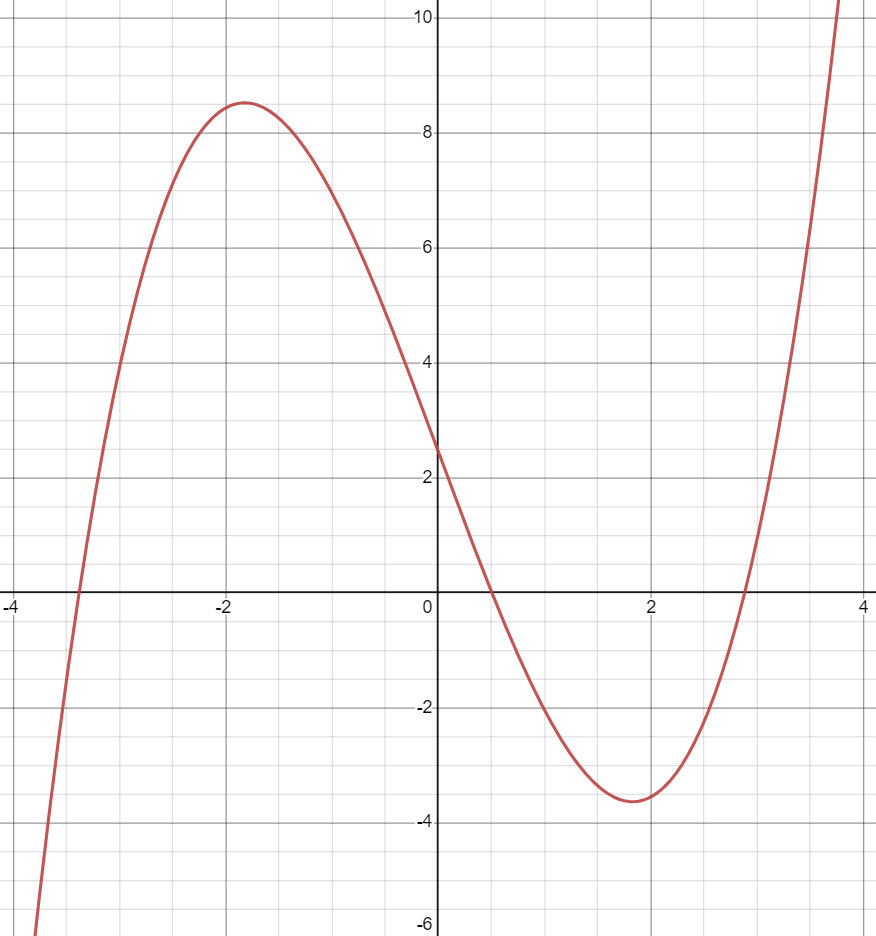
\includegraphics[scale=0.6, trim=0 80 0 50,clip]{cubic.png}
\end{center}
\begin{multicols}{2}
\begin{enumerate}[label= (\alph*)]
\item When is $f(x)$ increasing (when reading left to right)?\\\\\\\\
\item When is $f(x)$ decreasing?\\\\\\\\
\item When does $f(x)$ change between increasing and decreasing? What are the values of $f'(x)$ at those points?\\\\\\\\
\item Using tangent lines: which quantity is bigger $f'(2)$ or $f'(4)$?
\item Is $f'(x)$ increasing on $[2,4]$?\\\\\\\\\\
\item Find an interval where $f'(x)$ in decreasing.\\\\\\\\\\\\
\item Find a value of $x$ where $f'(x)$ change from decreasing to increasing?\\\\\\\\
\end{enumerate}
\end{multicols}
\newpage


\end{document}
